\begin{filecontents}{preliminary.sty}
\ProvidesPackage{preliminary}
%\DeclareOption{draft}{%
  \AtBeginDocument{%
    \renewcommand\maketitlehookc
\ProcessOptions
\RequirePackage{titling}
\endinput
\end{filecontents}

\documentclass[12pt, a4paper]{article}
\usepackage{setspace}
\usepackage{ragged2e}
\usepackage[centertags,reqno]{amsmath}
\usepackage{amssymb}
\usepackage{graphics,subfigure}
\usepackage[dvips]{graphicx}
\usepackage[dvipsnames]{xcolor}
\usepackage[hidelinks]{hyperref}
\usepackage{appendix}
\usepackage{natbib}
\usepackage{verbatim,color}
\usepackage{pdflscape}
\usepackage[showframe=false]{geometry}
\usepackage{changepage}
\usepackage{xcolor}
\usepackage{eurosym}
\usepackage{textcomp}
\usepackage[open,openlevel=1]{bookmark}
\usepackage{multirow}
\usepackage{caption}
\usepackage{hyphenat}
\usepackage{listings} % To include a Stata .do file
\usepackage{pdfpages} % To include the instructions from a pdf file
\newcommand{\mybox}[2]{{\color{#1}\fbox{\normalcolor#2}}}
\doublespacing

% Exception to hyphenation
\hyphenation{par-ti-ci-pants}
\hyphenation{par-ti-ci-pant}
\hyphenation{Hy-po-the-sis}
\hyphenation{ex-pe-ri-ment}
\hyphenation{ex-pe-ri-ments}

% Allows bigger tables to be scaled down
\usepackage{adjustbox}

%From my paper with Raymond
\usepackage{tabularx,calc}
\usepackage{dcolumn}                    % Aligns tables on the decimal point
\newcolumntype{d}[1]{D{.}{.}{#1}}       %       Aligns on dot
\newcolumntype{.}{D{.}{.}{3.5}}         %       Somehow it works better
\newcolumntype{C}{@{\extracolsep{.6cm}}c@{\extracolsep{0pt}}}
\usepackage{threeparttable}
\usepackage{siunitx,booktabs}
\sisetup{
    detect-all,
    round-integer-to-decimal = true,
    group-digits             = true,
    group-minimum-digits     = 4,
    group-separator          = {\,},
    table-align-text-pre     = false,
    table-align-text-post    = false,
    input-signs              = + -,
    input-symbols            = {*} {**} {***},
    input-open-uncertainty   = ,
    input-close-uncertainty  = ,
    retain-explicit-plus
}

% Commands to name appendices Appendix A, Appendix B, etc.
\makeatletter
%% The "\@seccntformat" command is an auxiliary command
%% (see pp. 26f. of 'The LaTeX Companion,' 2nd. ed.)
\def\@seccntformat#1{\@ifundefined{#1@cntformat}%
   {\csname the#1\endcsname\quad}  % default
   {\csname #1@cntformat\endcsname}% enable individual control
}
\let\oldappendix\appendix %% save current definition of \appendix
\renewcommand\appendix{%
    \oldappendix
    \newcommand{\section@cntformat}{\appendixname~\thesection\quad}
}

%Adds text specifying it is a preliminary version
%\usepackage{preliminary}

\title{Testing the Elicitation Procedure \\ of the Minimum Acceptable Probability \\
\Large Pre-Analysis Plan}
\author{Maria Polipciuc\thanks{Maastricht University. Email: \url{m.polipciuc@maastrichtuniversity.nl}. We thank Elias Tsakas and participants in the BEELab proposal meeting for valuable comments.} \and Martin Strobel\footnotemark[1]}
\date{\today	\vspace{1cm}}
\titlepage


\begin{document}
\begin{titlepage}
\clearpage
\maketitle
\thispagestyle{empty}
\end{titlepage}
\tableofcontents





%\emph{\section{Main page description (public)}
%\large \textcolor{RoyalBlue}{\textbf{Interventions}}
%
%\normalsize \noindent \textcolor{NavyBlue}{\textbf{Intervention(s)}}
%
%We compare minimum acceptable probabilities (MAPs) for which a participant prefers a binary lottery to a sure payoff across treatments within individual.
%Individuals have to decide in randomized order in three scenarios (treatments).
%The treatments keep the sure payoff and the payoffs of the lottery fixed, but vary the distribution of the winning probability of the lottery.
%
%\noindent \textcolor{NavyBlue}{\textbf{Trial Start Date}}
%
%Not applicable
%
%\noindent \textcolor{NavyBlue}{\textbf{Intervention Start Date}}
%
%June 2021
%
%\noindent \textcolor{NavyBlue}{\textbf{Intervention End Date}}
%
%June 2021
%
%
%
%\large \noindent \textcolor{RoyalBlue}{\textbf{Primary Outcomes}}
%
%\normalsize \noindent \textcolor{NavyBlue}{\textbf{Primary Outcomes (end points)}}
%
%MAPs
%
%\noindent \textcolor{NavyBlue}{\textbf{Primary Outcomes (explanation)}}
%
%The MAPs are elicited as thresholds for preferring a lottery to a sure payoff. 
%
%
%
%\large \noindent \textcolor{RoyalBlue}{\textbf{Experimental Design}}
%
%\normalsize \noindent \textcolor{NavyBlue}{\textbf{Experimental Design}}
%
%We elicit MAPs in an online experiment in a lottery similar to the \textit{Decision Problem} in \cite{Bohnet2004}.
%\cite{Bohnet2004} find that participants require a premium for being willing to trust someone compared to taking an equally risky bet with the same payoff externalities for an uninvolved person.
%They attribute this premium to betrayal aversion---an anticipatory disutility from being betrayed.
%
%In this study, we experimentally test a confounding explanation for this premium.
%We test whether participants' MAPs vary systematically as a result of the underlying distribution from which the probability of success of the lottery is drawn.
%We exogenously manipulate participants' probabilistic beliefs about this distribution by varying the different objective distributions of the winning probability.
%
%We then compare the resulting MAPs across treatments.
%We also compare the magnitude of the treatment effects with the effects in \cite{Bohnet2004,Bohnet2008}.
%
%\noindent \textcolor{NavyBlue}{\textbf{Experimental Design Details}}
%
%See the pre-analyis plan
%
%\noindent \textcolor{NavyBlue}{\textbf{Randomization Method}}
%
%Computer
%
%\noindent \textcolor{NavyBlue}{\textbf{Randomization Unit}}
%
%Individual
%
%\noindent \textcolor{NavyBlue}{\textbf{Was the treatment clustered?}}
%
%No
%
%\noindent \textcolor{NavyBlue}{\textbf{Planned Number of Observations}}
%
%450 (based on sample size calculations in Appendix \ref{section:appendixc})
%    
%\noindent \textcolor{NavyBlue}{\textbf{Was IRB approval obtained (only for ``In Development" and ``On-going" trials)?}} If so, also
%
%Yes.
%
%        IRB Name: Ethical Review Committee Inner City Faculties
%        
%        IRB Approval Date: June 9, 2021
%        
%        IRB Approval Number: ERCIC\_264\_08\_06\_2021}
        


\section{Introduction}
The Minimum Acceptable Probability (MAP) is a threshold value for preferring to trust someone over accepting a sure payoff.
It is elicited through a procedure similar to a Becker-De Groot-Marschak mechanism \citep{Becker1964} (expressed as a required probability or absolute number of favorable outcomes).

The concept was introduced by \cite{Bohnet2004} and it has been used—with slight variations—to elicit a determinant of trust, betrayal aversion, in a difference-in-difference design.
\cite{Bohnet2004} find that participants require a premium for being willing to trust someone compared to taking an equally risky bet with the same payoff externalities for an uninvolved person.
They attribute this premium to betrayal aversion---an anticipatory disutility from being betrayed.

As \cite{Li2020a} note, this attribution rests on the assumption that participants are rational expected utility maximizers.
Should participants not be rational expected utility maximizers, there are several possible confounding explanations for the premium found by \cite{Bohnet2004} and subsequent studies, such as ``ambiguity attitudes, complexity, different beliefs, and dynamic optimization'' \citep[p.~275]{Li2020a}.

In this study, we test experimentally what the contribution of one such confounding explanation is to this premium.
Specifically, we test whether participants' MAPs change as a result of the underlying distribution from which the probability of success of the lottery is drawn.
We remove the social and strategic aspects of a trusting decision, and study the MAP for accepting a risky lottery.
The treatments exogenously vary the distribution of the winning probability, thus manipulating participants’ expectations about the lottery’s winning chances.


Below we present the sample selection procedure, the experimental design, and the empirical strategy.



\section{Research Strategy}
This project will collect experimental data on an online platform dedicated to academic research (Prolific) in June 2021. Participants will be exposed to three treatments sequentially, in randomized order.
In each of the treatments, participants have to state the MAP for which they prefer a lottery to a sure payment.
%This is a version of \citeauthor{Bohnet2004}'s (\citeyear{Bohnet2004}) \textit{Decision Problem} (p. 469).
%The treatments differ in the underlying distribution from which the lottery is drawn.
%Given the complexity of the task, we will recruit participants with completed higher education, to increase the chances that task comprehension is not an issue.

The pre-analysis plan will be registered at the AEA RCT registry before the start of the data collection.


\subsection{Recruitment}
Participants are registered users on the online platform Prolific.
This platform is tailored for academic research, and gathers demographics about registered users.
We will send an invitation to the experiment only to participants who have completed higher education, to increase the chances that task comprehension is not an issue.
We will select as participants only residents of the United Kingdom.



\section{Design}
The study consists of three parts.
The first describes the tasks and asks comprehension questions.
This part pays a fixed payoff.
Only those who answer the comprehension questions correctly are allowed to continue to the second part, which is incentivized.
In this part we elicit participants' MAPs in three different scenarios.
After this, participants go through a survey (the third part), which is unincentivized.
We resolve uncertainty at the very end, when we inform participants about their payoff for the second part.

As mentioned above, participants in the experiment are asked to state their MAP in a \textit{Decision Problem} \citep{Bohnet2004}: what is their MAP for taking a gamble rather than accepting a sure payoff?
The experiment uses a within-subject design.\footnote{
We will also run a between-subject analysis using the data for the first decision participants make.
This is in order to check whether results in the within-subject analysis are not due to an experimenter demand effect.
The sample size calculation is based on the within-subject design.
For this reason, the main hypothesis refers to within-subject effects.
}
The complete instructions are available in Appendix \ref{section:appendixd}.

Below we present the main tasks and the post-experimental survey in more detail.


\subsection{Main tasks}
In each treatment, subjects face a different distribution of winning probabilities.
Each winning probability is represented by a wheel of fortune with 15 sectors.
Sectors are either dark blue (worth the high payoff of \pounds4) or light blue (worth the low payoff of \pounds1).
For their MAP, participants have to state an integer between 0 and 15.\footnote{
We chose to ask participants to state integers rather than probabilities because there is evidence that participants understand such questions better \citep[for instance, see Study 2 in][]{Quercia2016}.
}

Each of the three treatments consists of 32 different wheels, which can be ordered by the overall expected value over all wheels in the treatment.
We call the three treatments: the Good (the treatment with the highest expected value over all 32 wheels, where the distribution of the winning probability is left skewed), the Bad (the treatment with the lowest expected value over all 32 wheels, where the distribution of the winning probability is right skewed), and the Uniform (the expected value is in-between the ones in the other treatments, and the distribution of the winning probability is uniform).

The Bad and the Uniform distribution were chosen to reflect potential distributions imagined by participants in \cite{Bohnet2004} and \cite{Bohnet2008} in their \textit{Trust Game} and in their \textit{Decision Problem}, respectively.
Specifically, the Bad distribution has an expected probability of a dark blue sector over all 32 wheels of 0.2895, close to $p^*$ in their \textit{Trust Game}.
The Uniform distribution is plausibly what participants expected to face in their \textit{Decision Problem}: an overall probability of a dark blue sector over the 32 wheels of 0.5, with each possible winning probability being equally likely.

Payoffs are determined by a two-stage lottery.
In Stage 1, one of the 32 wheels is randomly drawn.
In Stage 2, the number of dark blue sectors in the randomly selected wheel is compared with the participant's MAP.
Should this number be equal to or exceed her MAP, the participant spins the virtual wheel for her payoff.
Should the number be lower than her MAP, the participant does not spin it.
She receives the intermediate safe payoff of \pounds2.

\begin{figure}[h!]
  \centering
 {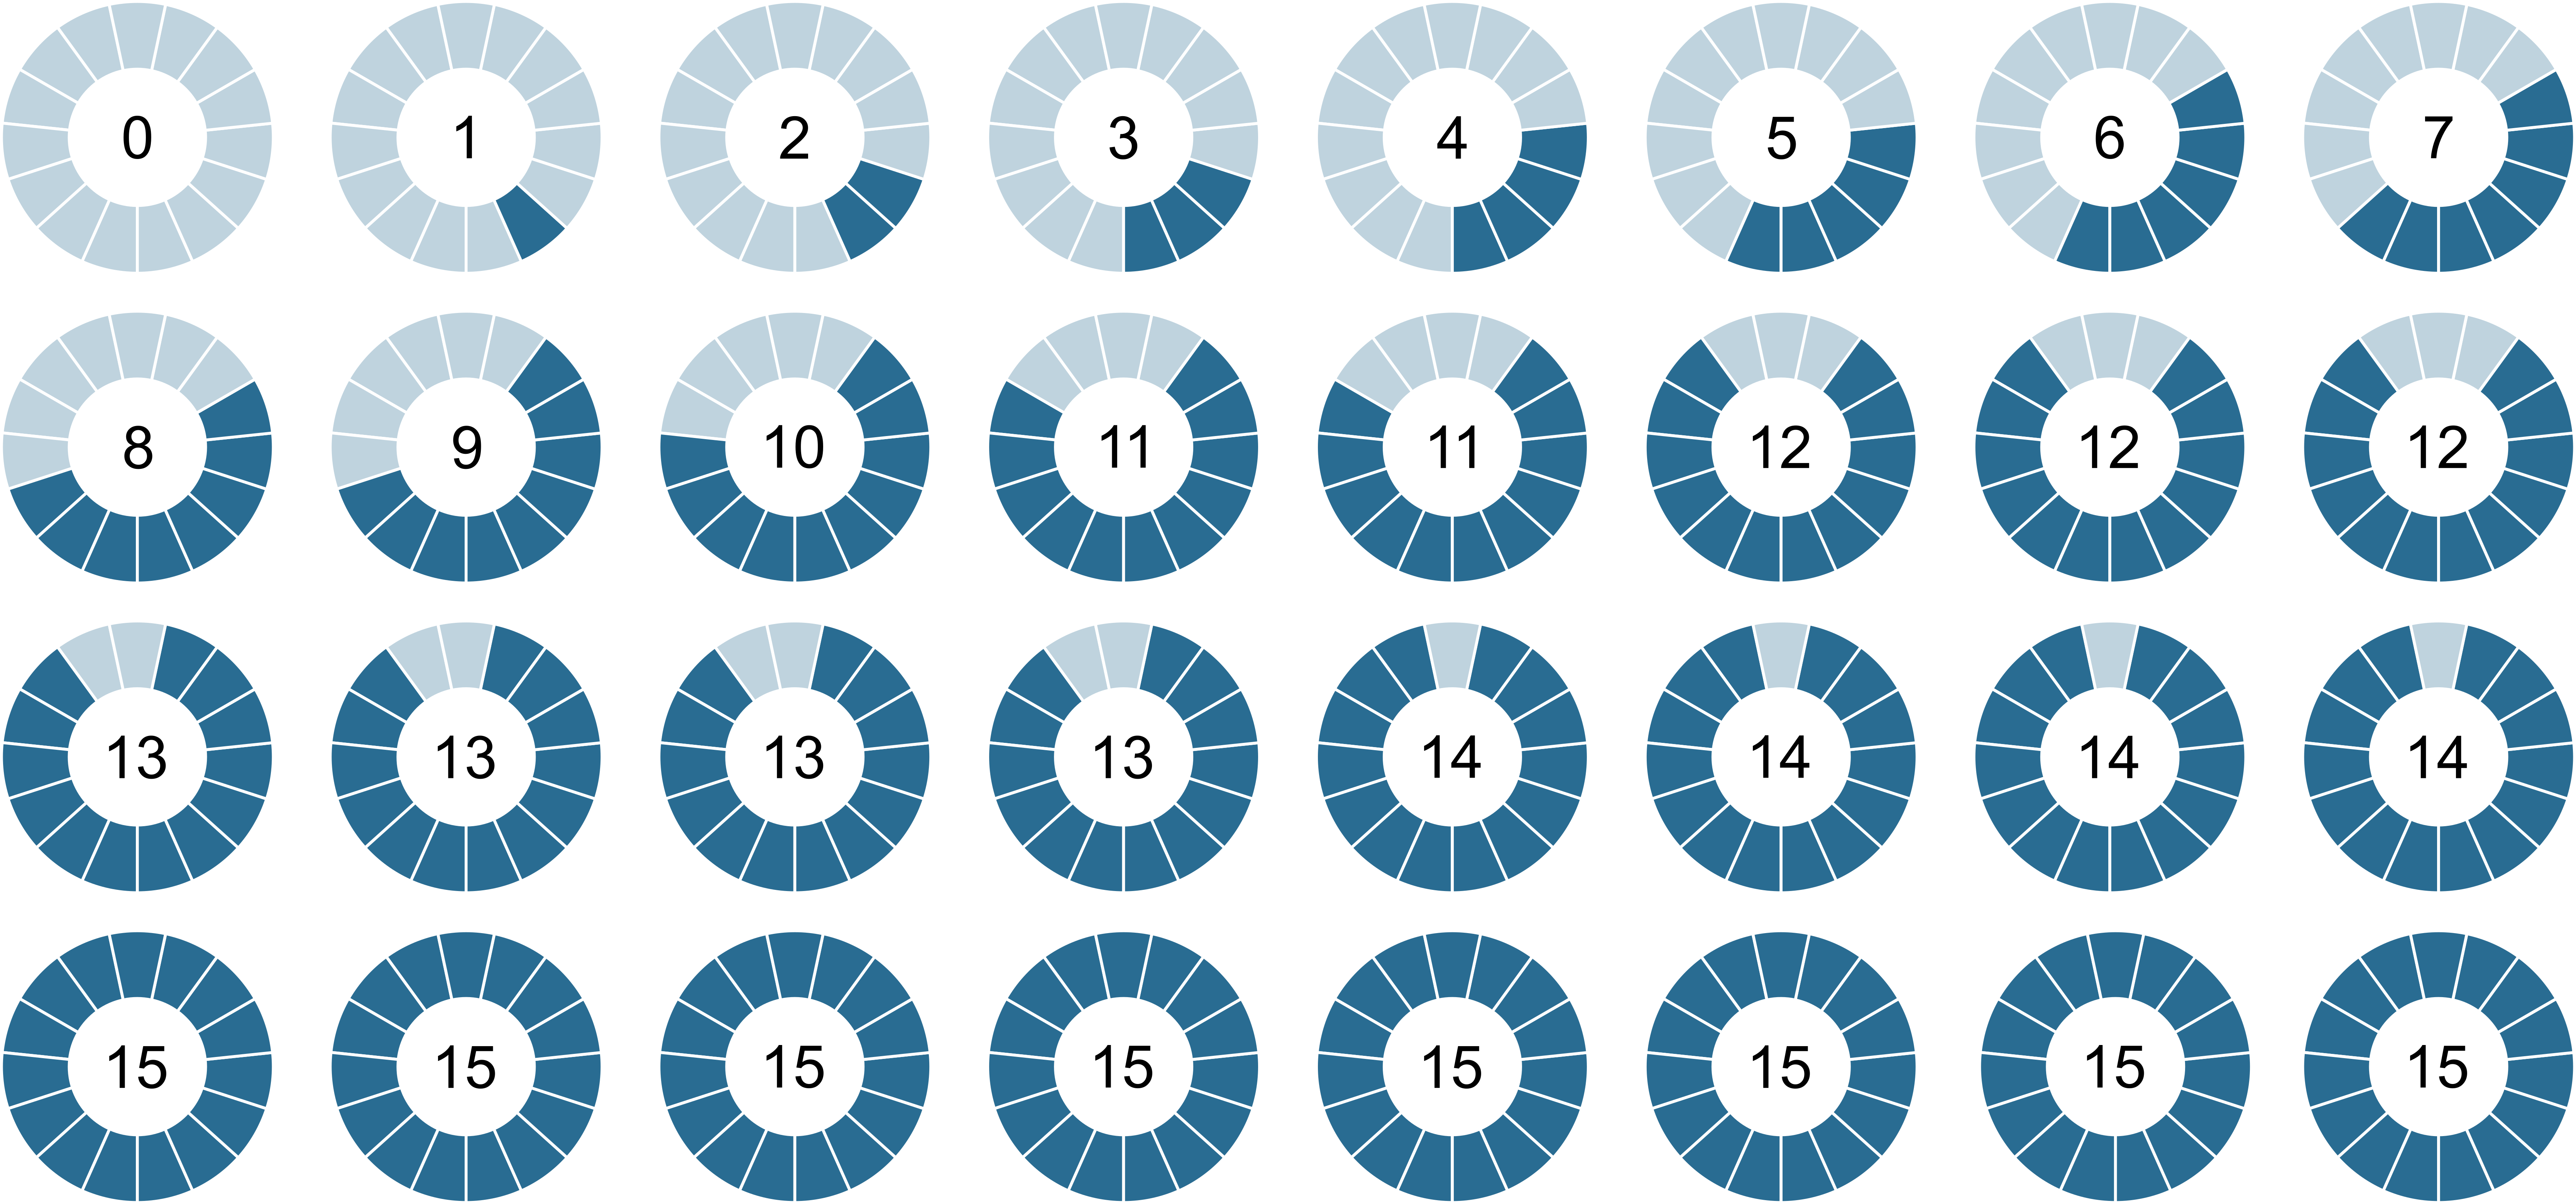
\includegraphics[width=0.95\linewidth]{Left_15.png}}
  \caption{Left skewed distribution (`The Good')}
  \label{fig:thegood}
\end{figure}


\begin{figure}[h!]
  \centering
 {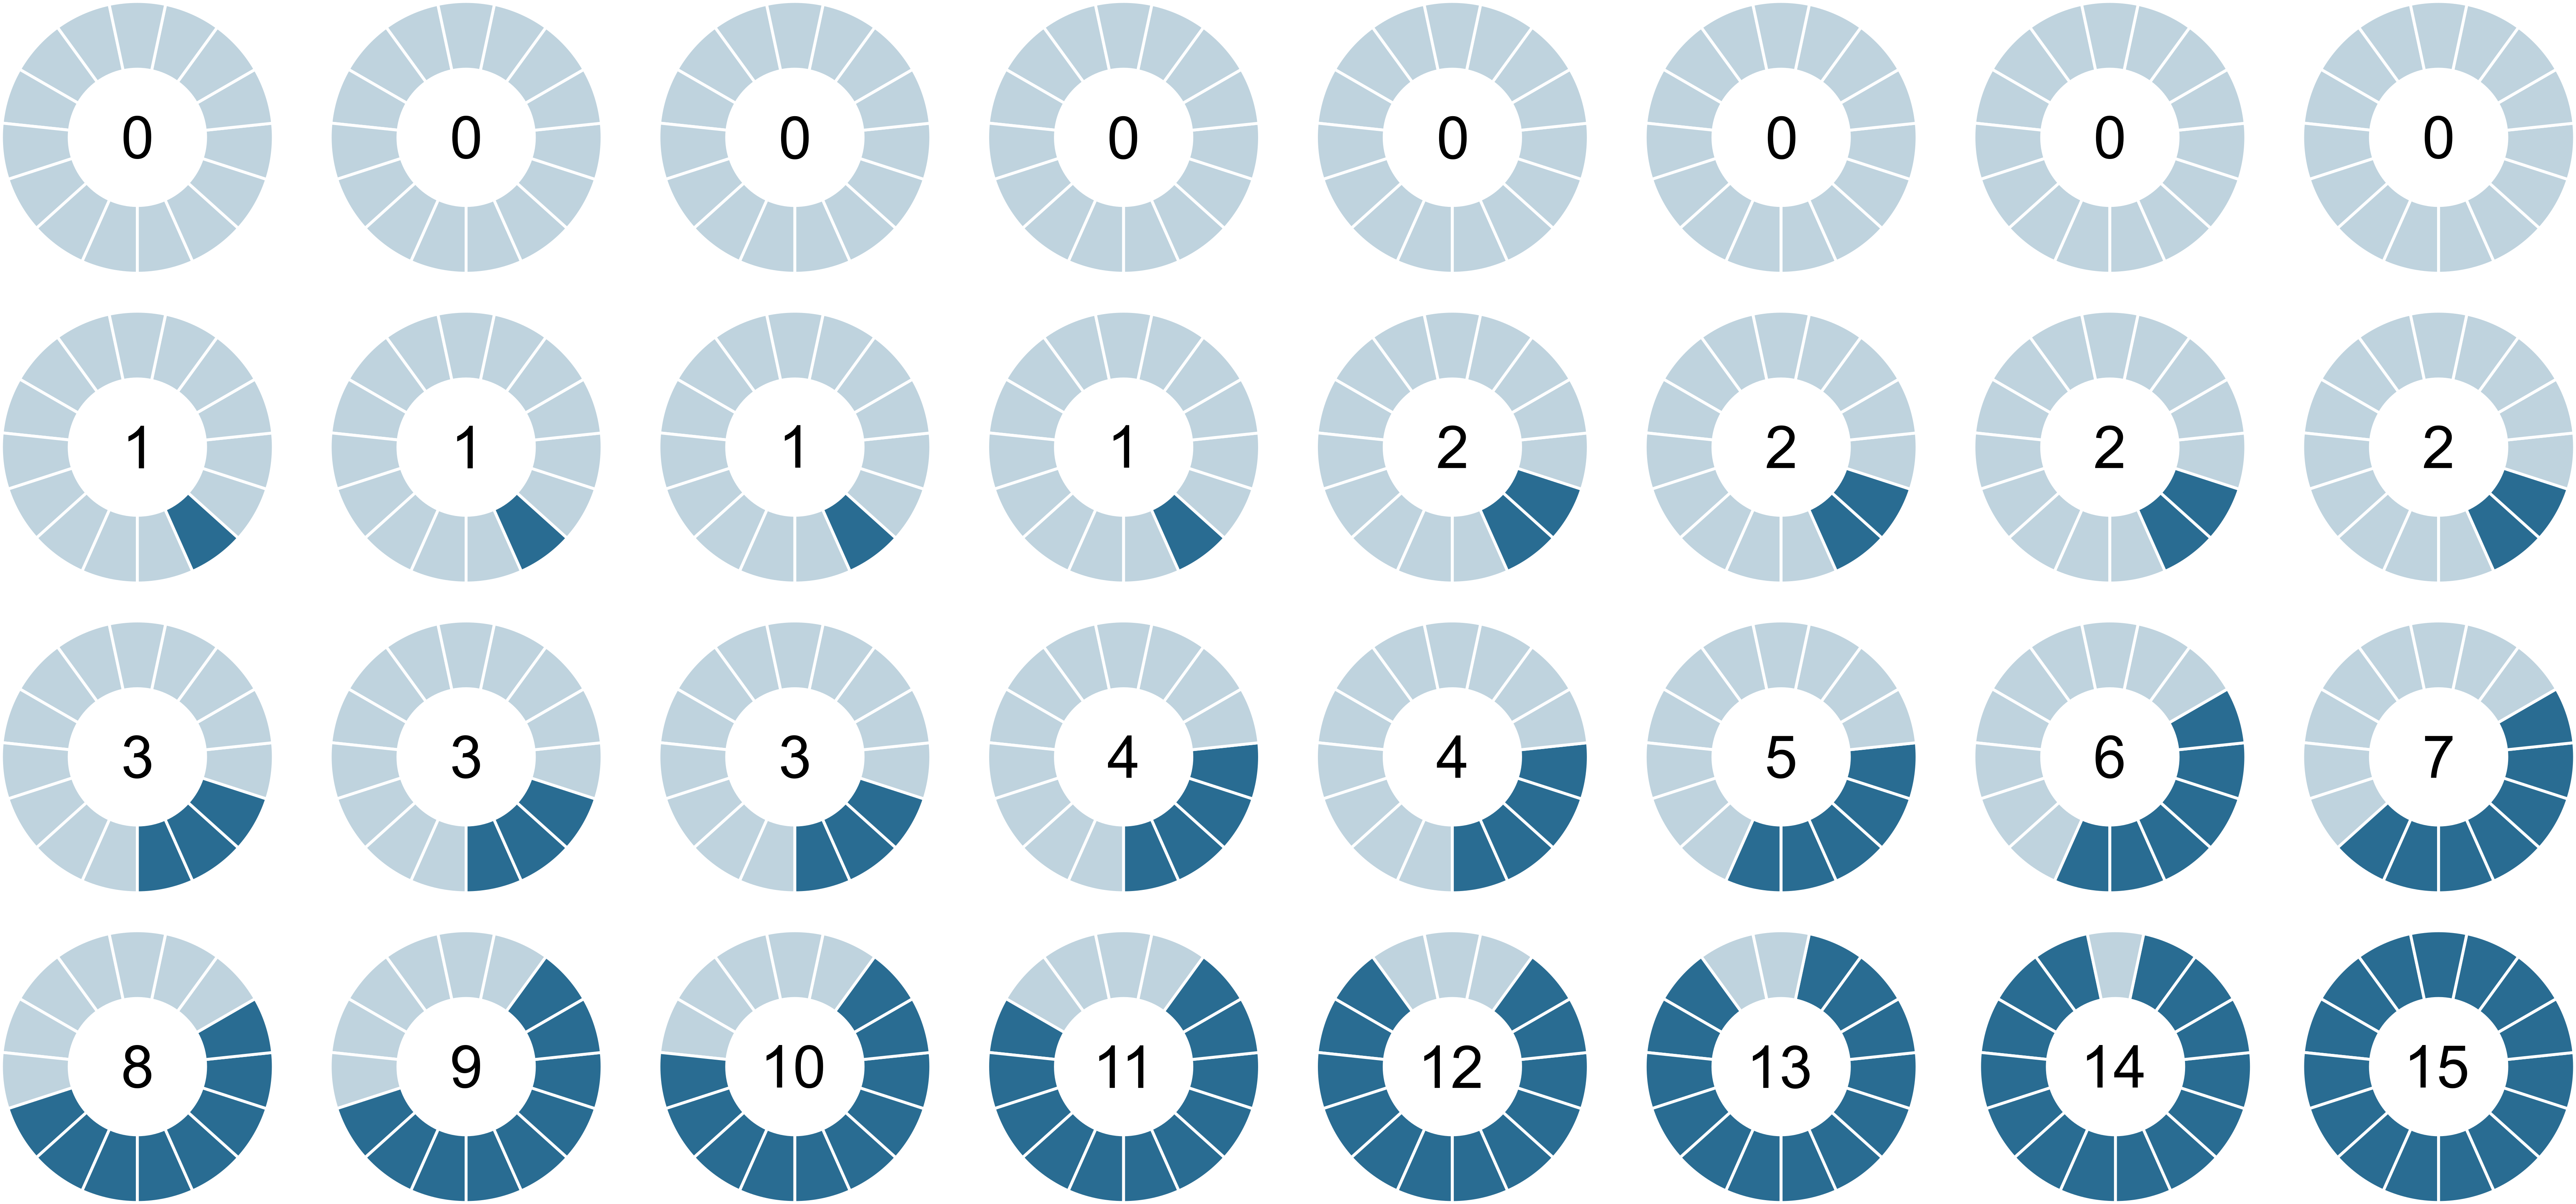
\includegraphics[width=0.95\linewidth]{Right_15.png}}
  \caption{Right skewed distribution (`The Bad')}
  \label{fig:thebad}
\end{figure}


\begin{figure}[h!]
  \centering
 {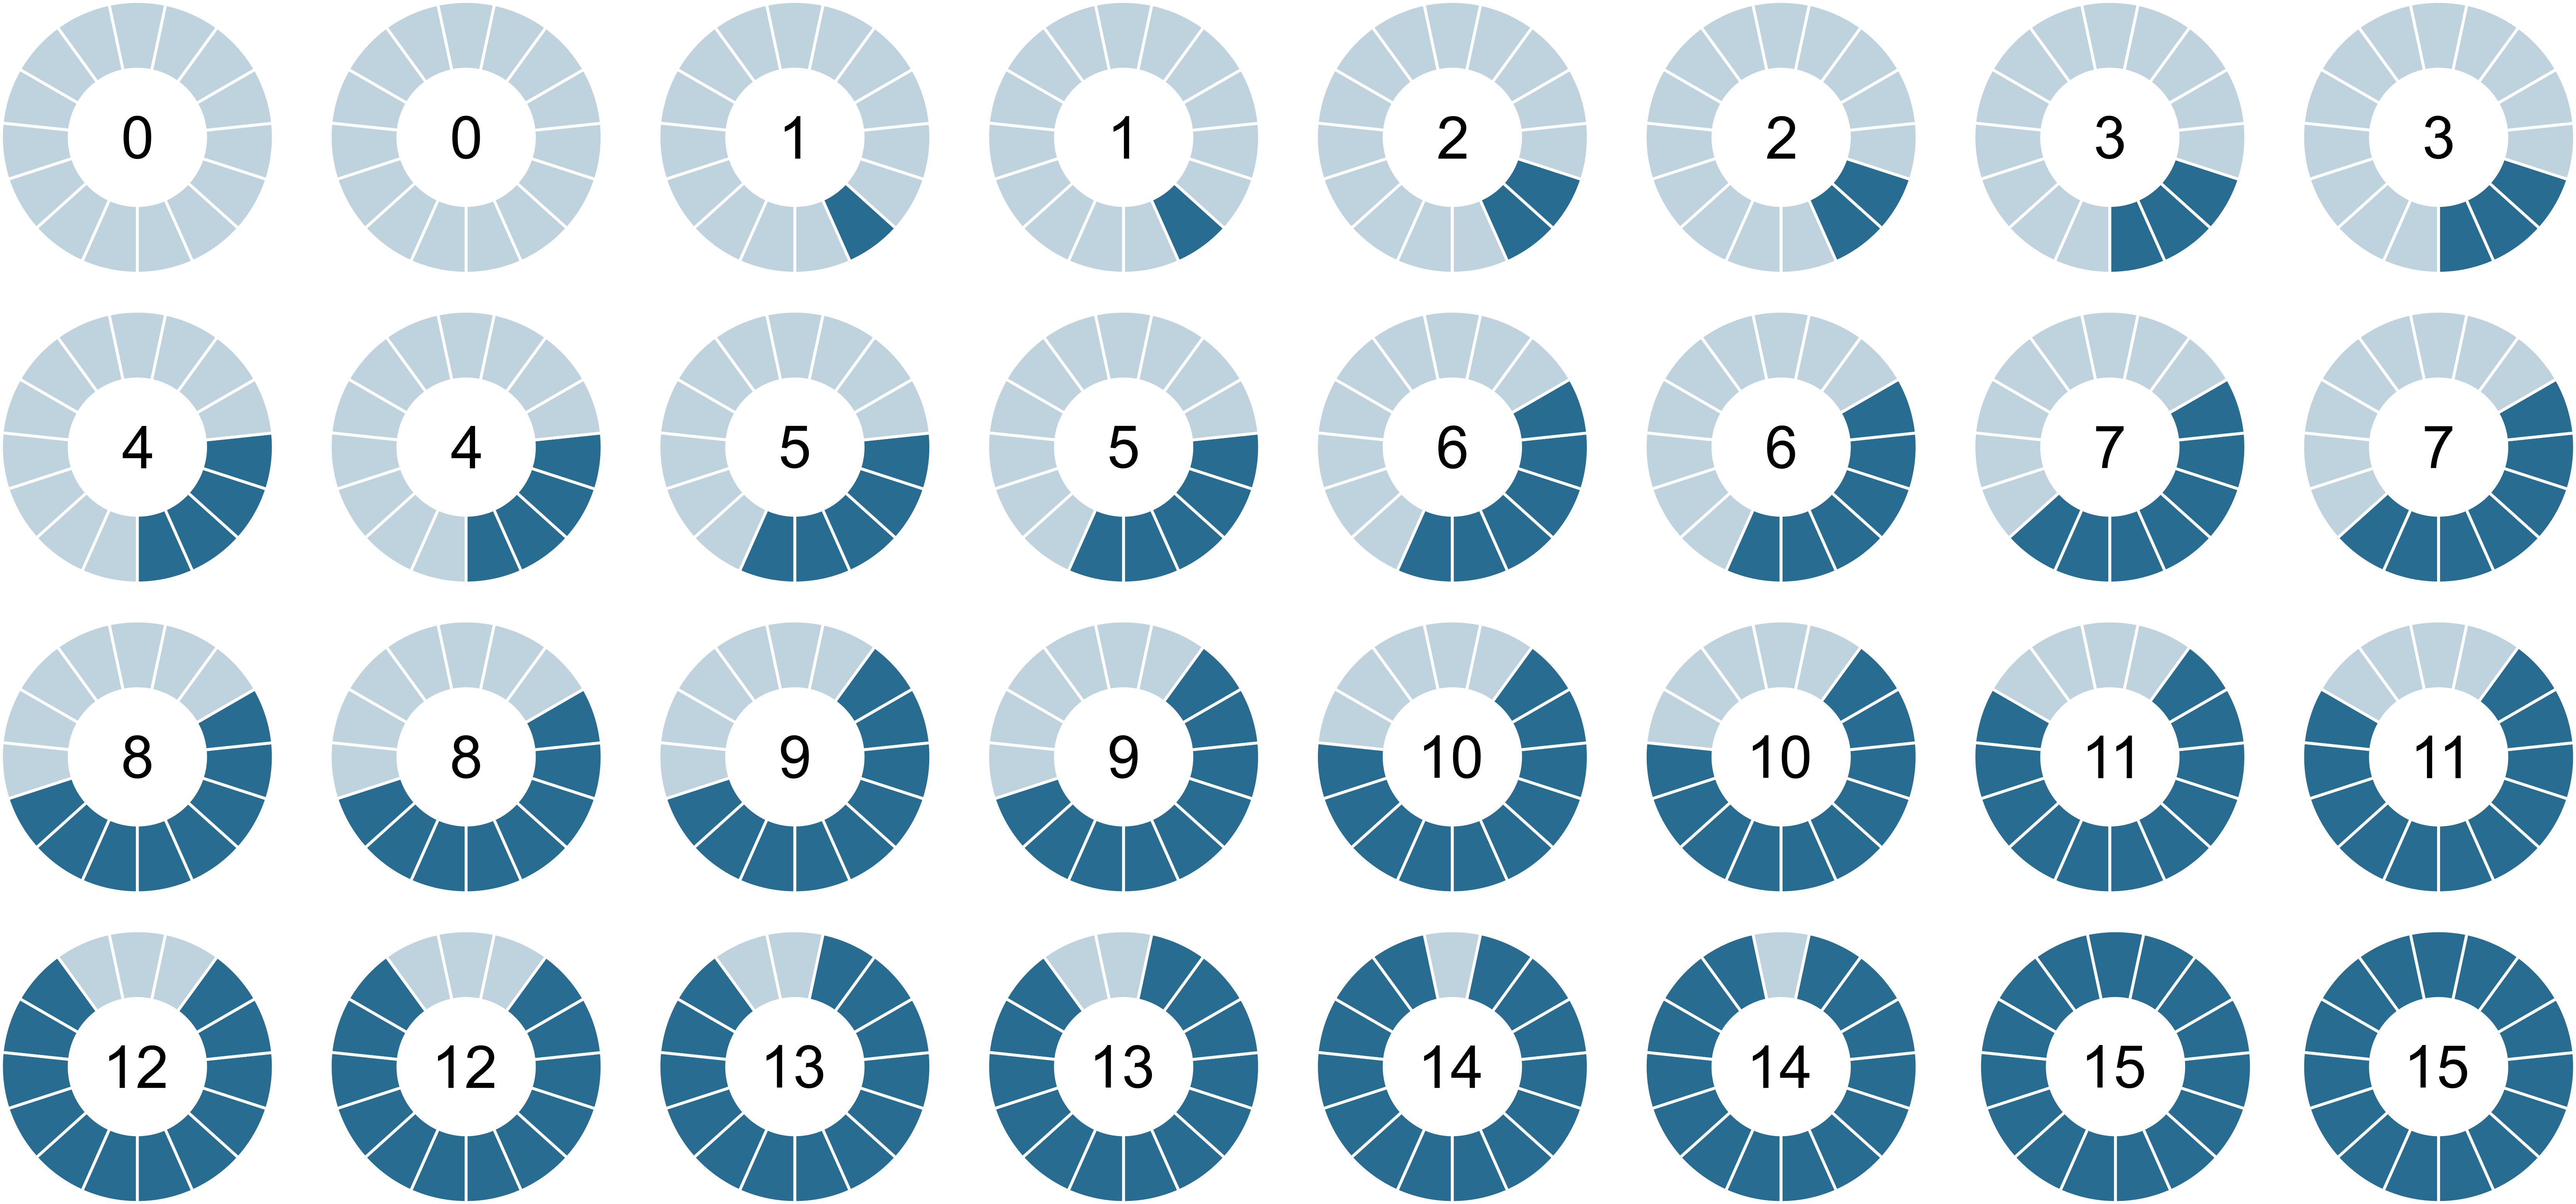
\includegraphics[width=0.95\linewidth]{Uniform_15.png}}
  \caption{Uniform distribution (`The Uniform')}
  \label{fig:theuniform}
\end{figure}

Participants who have answered the comprehension questions in Part 1 correctly see the pictures  in Figures \ref{fig:thegood}, \ref{fig:thebad}, \ref{fig:theuniform} in randomized order.
%\footnote{
%\textcolor{red}{The code for the spinning wheels is an adaptation of the wheel in: \url{https://github.com/tschiemer/qualtrics-gambling}, developed by Philip Tschiemer and Marc Hoeglinger.}
%}
Each picture is accompanied by the following text:

\textit{Consider the wheels above. Which wheels do you prefer to SPIN for your bonus?}

\textit{{\small Please enter an integer between 0 and 15.}}

\textbf{\textit{I prefer to SPIN wheels which have at least ... dark blue sectors.}}

\textit{If the randomly selected wheel has fewer than ... dark blue sectors, I DON'T SPIN it.
My bonus is \pounds2.}

\textit{If the randomly selected wheel has ... or more dark blue sectors, I SPIN it.
My bonus is}
\begin{itemize}
\item \textit{\pounds1 if the selected wheel lands on light blue, and}
\item \textit{\pounds4 if it lands on dark blue.}
\end{itemize}

Participants have to fill in the text in the bold italicized sentence (which is not bold nor italicized in the version participants see).
The rest of the `...' are automatically filled in (and/or updated) with the participant's input.

\subsection{Survey questions}
Participants answer the following type of questions:
\begin{itemize}
\item a question similar to the main tasks, but which is unincentivized. This question elicits their MAP in an ambiguous situation;
\item an adapted cognitive reflection test \citep{Frederick2005,Thomson2016};
\item a question about the subject they studied for their most recent degree;
\item a general risk taking question \citep{Dohmen2011};
\item a question about their aspiration level for earnings from participating in a survey;
\item a couple of questions to check their anchoring susceptibility, from which an anchoring score can be computed \citep{Cheek2017};
\item a set of questions about their optimism/pessimism, the revised Life Orientation Test \citep{Scheier1994};
\item a brief sensation seeking scale, BSSS-4 \citep{Stephenson2003}.
\end{itemize}

Additional information will be requested from Prolific, who can provide data on participants' age, gender, subject for which they received their most recent degree, whether participants make household spending decisions, and investment behavior.




\section{Empirical Strategy}
Should participants be expected utility maximizers, their MAPs should not differ between the three treatments.
This would be in line with what \cite{Bohnet2004} and \cite{Bohnet2008} assume.

In their Appendix A, \cite{Li2020a} show by means of a numerical example that if participants are not expected utility maximizers, ambiguity aversion alone could generate the pattern attributed to betrayal aversion.
Since there is evidence that attitudes towards complex risks and attitudes towards ambiguity are correlated \citep{Armantier2016}, we redo their numerical exercise for our three distributions: the Good, the Bad, and the Uniform in Appendix \ref{section:appendixa}.
For this calculation we assume that participants view the tasks as complex risky situations---and this underlies their inverse-s-shaped probability weighting.

The calculation leads to the main hypothesis below.



\subsection{Hypotheses}
\subsubsection{Main hypothesis}
\noindent \textbf{Hypothesis 1} \quad \textit{The MAP in the Good treatment (more mass on high values of $p^*$) is lower than the MAP in the Uniform treatment (a uniform distribution over $p^*$), which is lower than the MAP in the Bad treatment (more mass on low values of $p^*$).}

\begin{equation}
MAP_G < MAP_U < MAP_B
\end{equation}

An alternative hypothesis is that the MAP ordering is precisely the opposite of the one in H1.
A reason for this alternative hypothesis is that participants possibly anchor their MAP on the visual cues offered by a distribution.
That is, they require a higher MAP the higher the overall winning probability over the 32 wheels.
If this explanation is true, we should see the reverse ordering to the one in H1, and a positive correlation between one's anchoring score and (i) displaying this reverse ordering and (ii) the effects' absolute value (both $|MAP_G - MAP_U|$ and $|MAP_B - MAP_U|$).


\subsubsection{Secondary hypotheses}
Since the MAP is a way to gauge (complex) risk aversion, we expect that in the same treatment females state higher MAPs than males on average.

\noindent \textbf{Hypothesis 2} \quad \textit{Within each treatment, females require higher MAPs on average than males.}

Some of the within-subject differences between treatments could be due to difficulties in assessing complex risks.
Should this be the case, we expect participants scoring lower on the CRT tasks to have higher variance in their MAPs.

\noindent \textbf{Hypothesis 3} \quad \textit{Within individuals, the variance in MAP correlates negatively with the CRT score.}

Individuals might derive utility from spinning the wheels in the tasks.
We expect those who score higher on sensation seeking to also have lower MAPs on average in each treatment.

\noindent \textbf{Hypothesis 4} \quad \textit{Within each treatment, participants who score high on sensation seeking require lower MAPs on average than those who score low.}

Several papers find that higher aversion to complex risks is positively correlated with higher ambiguity aversion \citep{Halevy2007,Armantier2016}.
The numerical example in Appendix \ref{section:appendixa} suggests the following hypothesis.

\noindent \textbf{Hypothesis 5} \quad \textit{Within individuals, higher effect sizes (in absolute terms, $|MAP_G - MAP_U|$ and $|MAP_B - MAP_U|$) are positively correlated with a higher ambiguity aversion ($MAP_A - MAP_U$).}

Finally, there are two concepts for which we do not have clear directional hypotheses.
We will explore the relation between the MAPs and optimism/pessimism, as well as that between the MAPs and an aspiration level for earnings.




\subsection{Specifications and Analysis}
We present the OLS regressions which will be used to test the main hypothesis.
Additionally, we will also run appropriate non-parametric tests.

The main hypothesis will be tested using the following regression:
\begin{equation} \label{eq:1}
MAP_i = \beta + \beta_G \times G + \beta_B \times B + \epsilon_i
\end{equation}

\noindent where $MAP_i$ is the MAP chosen by participant $i$, $G$ is an indicator which takes the value of 1 if the decision was made in the Good treatment, $B$ is an indicator which is 1 if the decision was made in the Bad treatment and $\epsilon_i$ is a random error term.
Standard errors in the estimation will be clustered at the individual level.

For Hypothesis 2, all terms will be interacted with indicator variable $F_i$, which takes the value 1 if the participant is female:
\begin{equation} \label{eq:2}
MAP_i = \beta + \beta^F \times F_i + \beta_G \times G + \beta_G^F \times G \times F_i + \beta_B \times B + \beta_B^F \times B \times F_i + \epsilon_i
\end{equation}

For Hypotheses 3--5, we will calculate Pearson's correlation coefficient between the variables pertaining to each hypothesis.

The formal statements of the hypotheses are in Appendix \ref{section:appendixb}.

\clearpage
\pagebreak
\bibliographystyle{apalike}
\bibliography{Communities}

\clearpage
\pagebreak

\appendix
\section{Numerical Example}
\label{section:appendixa}
\setcounter{figure}{0}
\setcounter{table}{0}
\renewcommand{\thefigure}{A.\arabic{figure}}
\renewcommand{\thetable}{A.\arabic{table}}

\cite{Li2020a} show in their Appendix A that---even in the absence of betrayal aversion---a different effect of ambiguity attitudes in the \textit{Risky Dictator Game} and in the \textit{Trust Game} of \cite{Bohnet2004} and \cite{Bohnet2008} may lead to the strategic premium observed in papers on betrayal aversion.

We apply their numerical example to the three distributions used in our study.
We make the following assumptions:
\begin{itemize}
\item the utility of outcomes is fixed. We consider $U(\pounds4) = 1$, $U(\pounds1) = 0$, and $U(\pounds2) = 1/3$;\footnote{
We set the utility of the safe payoff such that $U(\pounds2) = x \times U(\pounds4) + (1-x) \times U(\pounds1)$, where $x \in [0,1]$.
This leads to $x^* = 1/3$.
}
\item participants use a probability weighting function because they perceive the tasks to involve complex risks. Similar to \cite{Li2020a}, we use \citeauthor{Prelec1998}'s (\citeyear{Prelec1998}) \textit{compound invariance} function:
$$w(p) = (exp(-(-ln(p))^\alpha))^\beta$$ 
\item we use $\alpha = 0.65$ and $\beta = 1.0467$, which according to \cite{Li2020a} are the most common values for risky probability weighting;
\item participants use ``forward'' evaluation: they consider the three possible outcomes, and take into account their probabilities;
\item participants have the following rank-dependent utility function \citep{Schneider2019}:
$$RDU = w(P(\pounds4)) \times 1 + (w(P(\pounds4) + P(\pounds2)) - w(P(\pounds4))) \times (1/3)$$
where $P(\pounds4)$ is the probability of receiving the high payoff, $P(\pounds2)$ the probability of receiving the safe payoff, and $P(\pounds1)$ the probability of receiving the low payoff.
\end{itemize}

In this case, the MAPs which maximize participants' utility in the three treatments are: $MAP_G = 7$ ($RDU = 0.628$), $MAP_U = 8$ ($RDU = 0.495$), and $MAP_B = 9$ ($RDU = 0.439$).

\section{Hypothesis Testing}
\label{section:appendixb}
\setcounter{figure}{0}
\setcounter{table}{0}
\renewcommand{\thefigure}{B.\arabic{figure}}
\renewcommand{\thetable}{B.\arabic{table}}

\subsection{Hypothesis 1}
$H0: \beta_G = \beta_B = 0 \\
H1: \beta_G < 0 < \beta_B$

\subsection{Hypothesis 2}
Within each treatment:

\noindent $H0: \beta^F = 0 \\
H1: \beta^F > 0$

\noindent and

\noindent $H0: \beta^F + \beta_G^F = 0 \\
H1: \beta^F + \beta_G^F > 0$

\noindent and

\noindent $H0: \beta^F + \beta_B^F = 0 \\
H1: \beta^F + \beta_B^F > 0$

\subsection{Hypothesis 3}
Within individuals:

\noindent $H0: corr(var_{MAP},CRT) = 0 \\
H1: corr(var_{MAP},CRT) < 0$

\noindent where $var_{MAP}$ is the intra-individual variance of the MAP, as calculated from the respondent's $MAP_G$, $MAP_B$ and $MAP_U$.

\subsection{Hypothesis 4}
Within each treatment:

\noindent $H0: corr(MAP,BSSS4) = 0 \\
H1: corr(MAP,BSSS4) < 0$

\noindent where $BSSS4$ is the sensation seeking score, calculated as described in \cite{Cheek2017}.

\subsection{Hypothesis 5}
Within individuals:

\noindent $H0: corr(|MAP_G - MAP_U|,MAP_A - MAP_U) = 0 \\
H1: corr(|MAP_G - MAP_U|,MAP_A - MAP_U) > 0$

\noindent and

\noindent $H0: corr(|MAP_B - MAP_U|,MAP_A - MAP_U) = 0 \\
H1: corr(|MAP_B - MAP_U|,MAP_A - MAP_U) > 0$



\section{Sample size calculations}
\label{section:appendixc}
\setcounter{figure}{0}
\setcounter{table}{0}
\renewcommand{\thefigure}{C.\arabic{figure}}
\renewcommand{\thetable}{C.\arabic{table}}

The Stata code below builds heavily on Example 2 in \cite{CamposMercade2018}.
\lstinputlisting[basicstyle=\tiny]{Power_analysis_clean.do}


\section{Instructions}
\label{section:appendixd}
\setcounter{figure}{0}
\setcounter{table}{0}
\renewcommand{\thefigure}{D.\arabic{figure}}
\renewcommand{\thetable}{D.\arabic{table}}

In the notes for the experimenters, the Good distribution is referred to as `Left\_Skew' and the Bad as `Right\_Skew'.
Analogously, $MAP_G$ is referred to as `$MAP_L$' and $MAP_B$ as `$MAP_R$'.

The experiment will be run using Qualtrics.
The .qsf file is available \href{https://www.dropbox.com/s/2w1yv4px9pywuip/Wheelz.qsf?dl=0}{\textcolor{blue}{here}} (for help on importing a .qsf file into Qualtrics, check {\href{https://www.qualtrics.com/support/survey-platform/survey-module/survey-tools/import-and-export-surveys/#ImportingASurvey}{\textcolor{blue}{this Qualtrics support page}}).

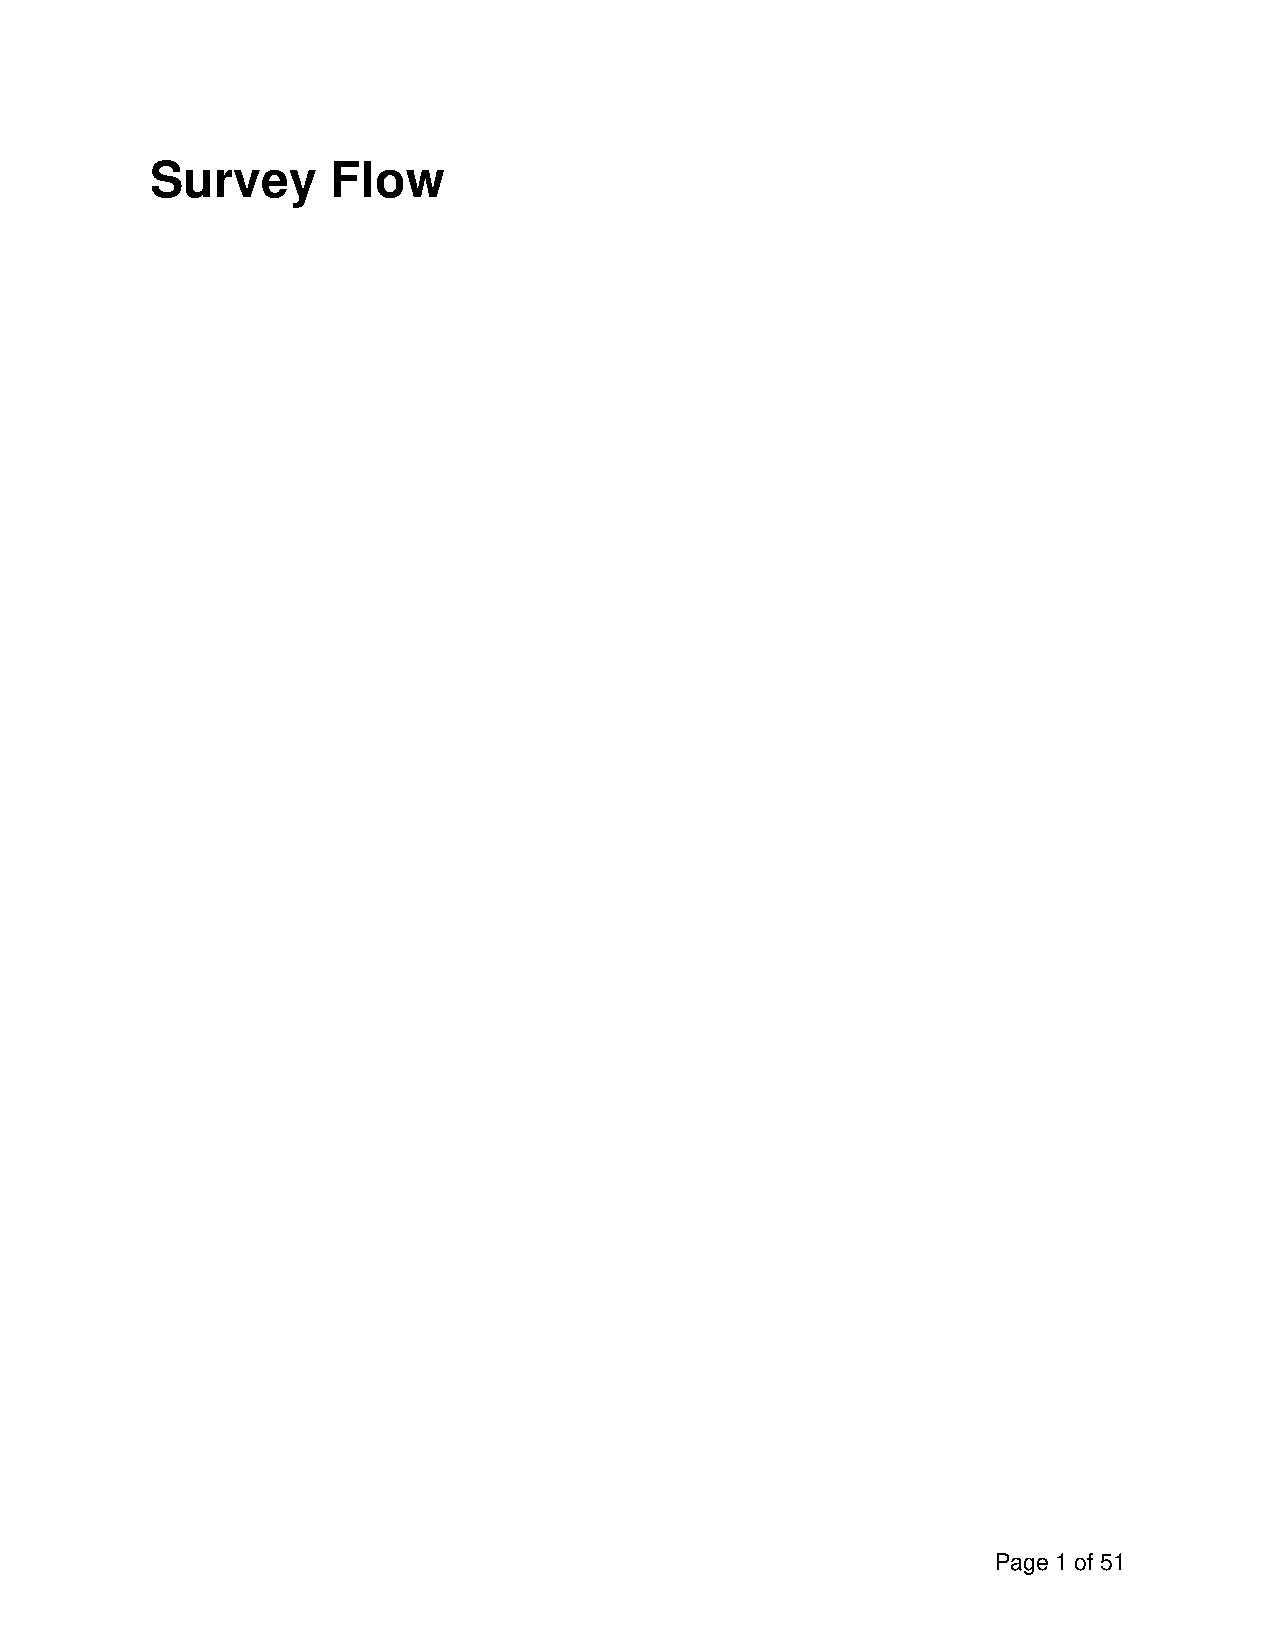
\includepdf[pages=1-,nup=1x2,landscape=true]{Instructions_Prolific.pdf}


\end{document}